\subsection{Валидация \texttt{nupropagator}}
 Проведем сравнение результатов, полученных с помощью двух програмнных пакетов: \texttt{nuFATE}~\cite{Vincent_2017} и \texttt{nupropagator}. Будем сравнивать потоки мюонного нейтрино, приходящих под разными углами после прохождения через землю в некоторой точке, находящейся на глубине 1 км от поверхности Земли. В качестве нейтринного потока на поверхности земли был использован степенной поток $E^{-2}$. Также построим переменную $\delta_{asymm}$ в зависимости от энергии, которая определяется следующим образом: 
 \begin{equation}
     \delta_{asym} = 2\frac{F^{nupropagator}_{\nu}(E,x) - F^{nuFATE}_{\nu}(E,x)}{F^{nupropagator}_{\nu}(E,x) +
     F^{nuFATE}_{\nu}(E,x)}
 \end{equation}
\begin{figure}[!h]
\centering
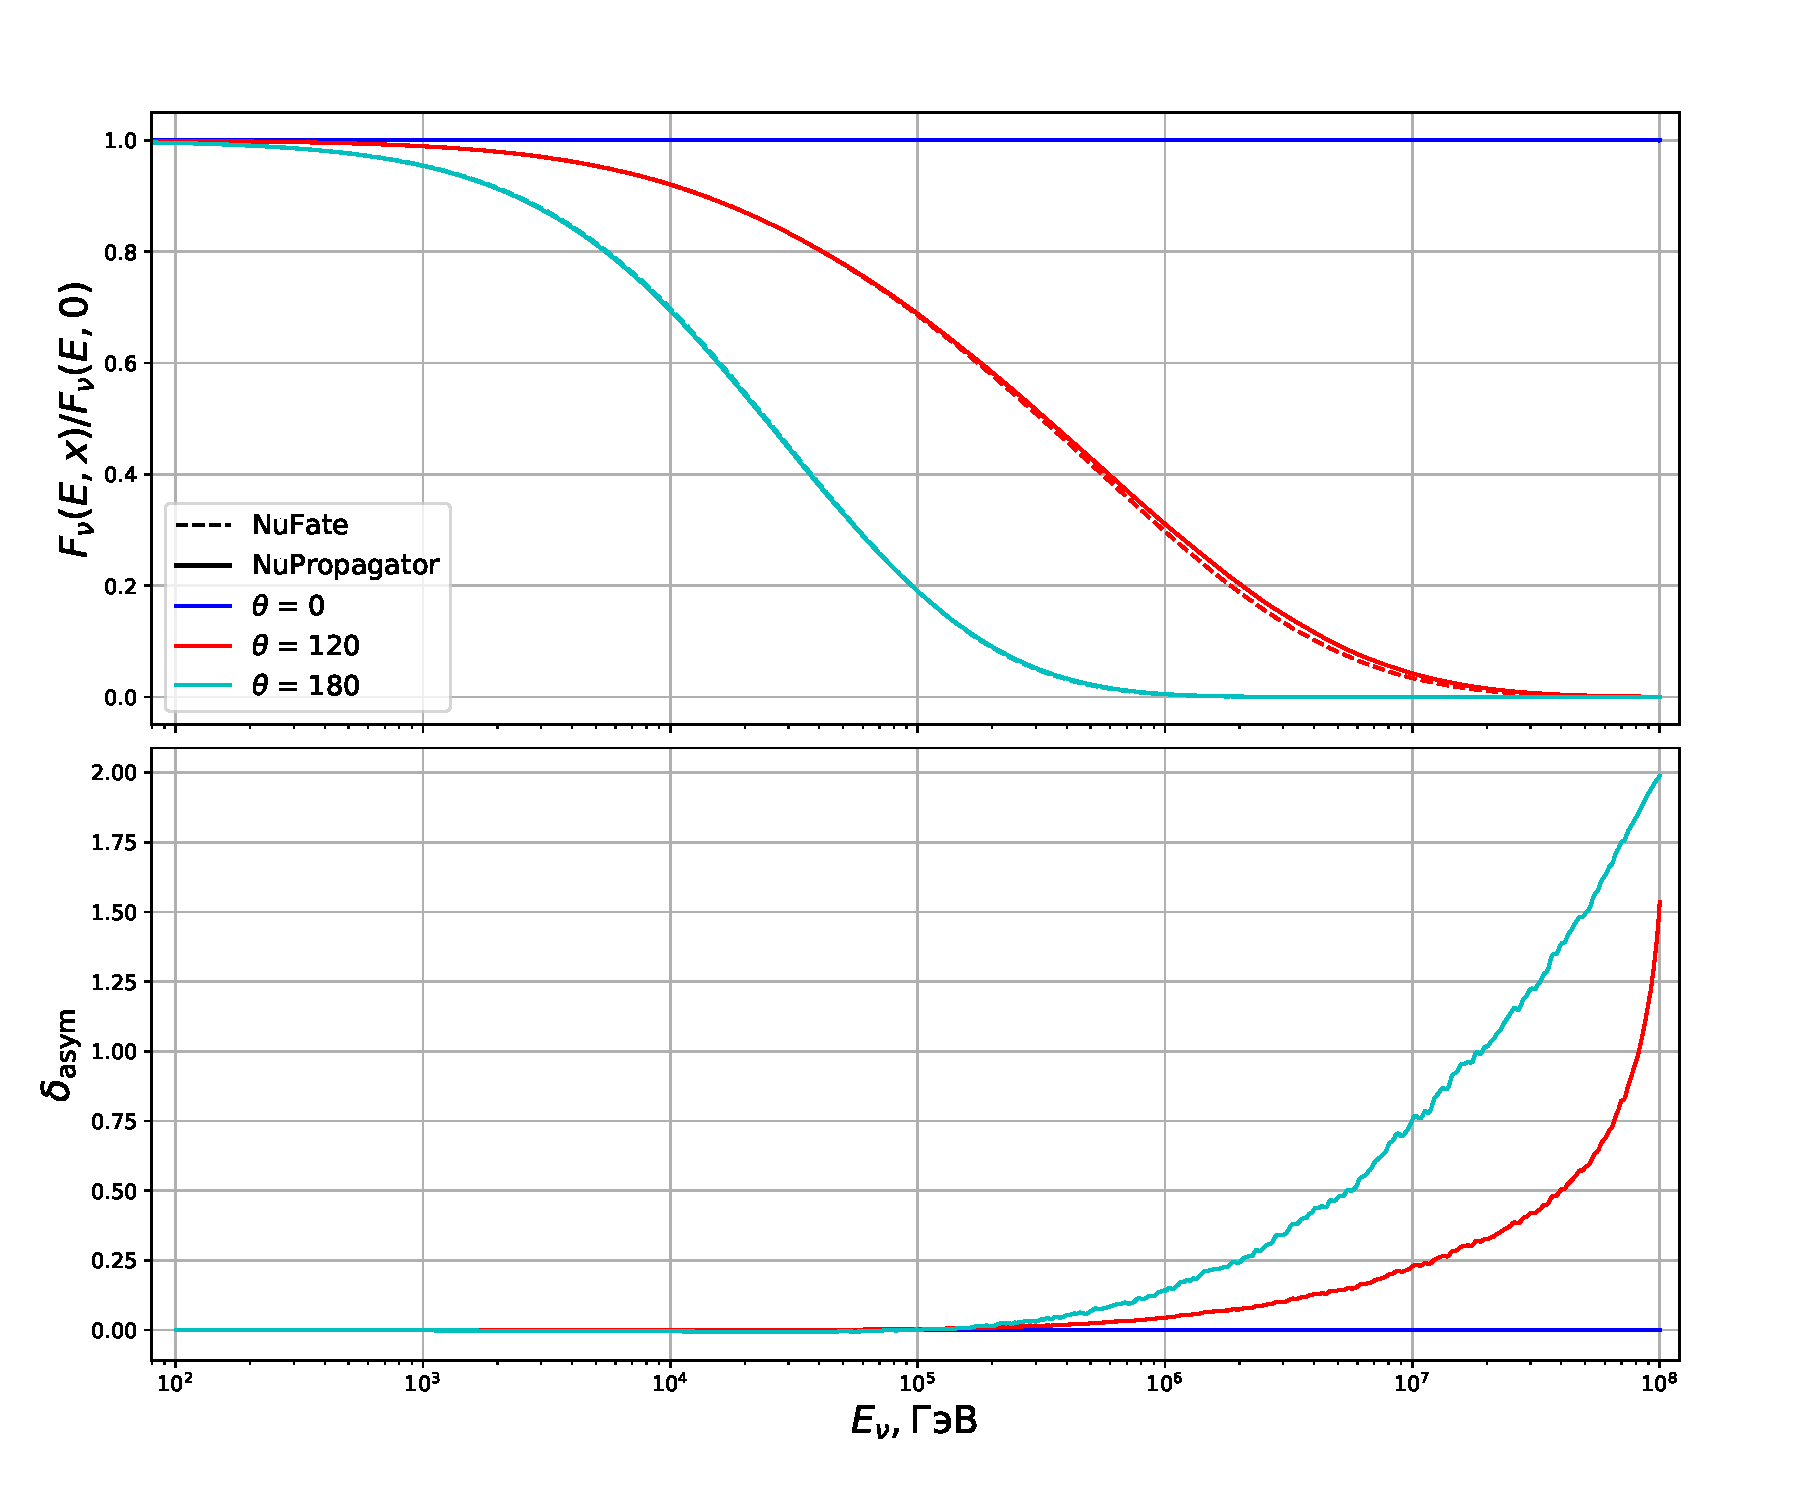
\includegraphics[width=\linewidth]{images/NuProp/compNuandNu.pdf}
\caption{Сравнение потоков, полученных с помощью \texttt{nuFATE} и \texttt{Nupropagator} для разных углов прилета нейтрино.}
\label{fig:flux_compare}
\end{figure}
Как можно видеть из рис.~\ref{fig:flux_compare} результаты находятся в хорошем согласии при энергиях меньше $10^6$ГэВ. Дальнейшее расхождение можно объяснить как отсутствием учета эффекта регенерации потоков за счет таонного нейтрино, различным поведением моделей сечений при больших энергиях, различными численными способами решения кинетических уравнений, которым описывается эволюция потоков нейтрино.   
